
\section{Metodologia}

A metodologia aplicada para o desenvolvimento do projeto Memória Viva foi dividida em cinco etapas principais: levantamento de requisitos, definição da arquitetura, desenvolvimento incremental, testes com usuários e validação com especialistas em saúde e tecnologia assistiva.

\subsection{Etapa 1: Levantamento de Requisitos}

Nesta fase, foram realizadas entrevistas com cuidadores, familiares e profissionais da saúde, a fim de identificar as principais dificuldades enfrentadas por idosos com Alzheimer ou DFT. A Tabela~\ref{tab:requisitos} apresenta uma síntese dos requisitos levantados.

\begin{table}[h]
\centering
\caption{Principais requisitos levantados com cuidadores}
\label{tab:requisitos}
\begin{tabular}{|p{5cm}|p{8cm}|}
\hline
\textbf{Necessidade} & \textbf{Solução proposta} \\ \hline
Reconhecimento rápido do idoso & Biometria facial embutida com câmera \\ \hline
Memórias personalizadas com afeto & Banco de dados com fotos, vídeos e áudios \\ \hline
Interação natural por voz & Uso da Web Speech API + IA generativa \\ \hline
Histórico de interações & Registro com data/hora e análise de humor \\ \hline
Painel para cuidadores & Dashboard web com autenticação segura \\ \hline
\end{tabular}
\end{table}

\subsection{Etapa 2: Arquitetura e Ferramentas}

A arquitetura da aplicação foi definida com base em tecnologias gratuitas, de fácil integração e com bom suporte comunitário. A Figura~\ref{fig:arquitetura} mostra a visão geral da arquitetura adotada.

\begin{figure}[h]
\centering
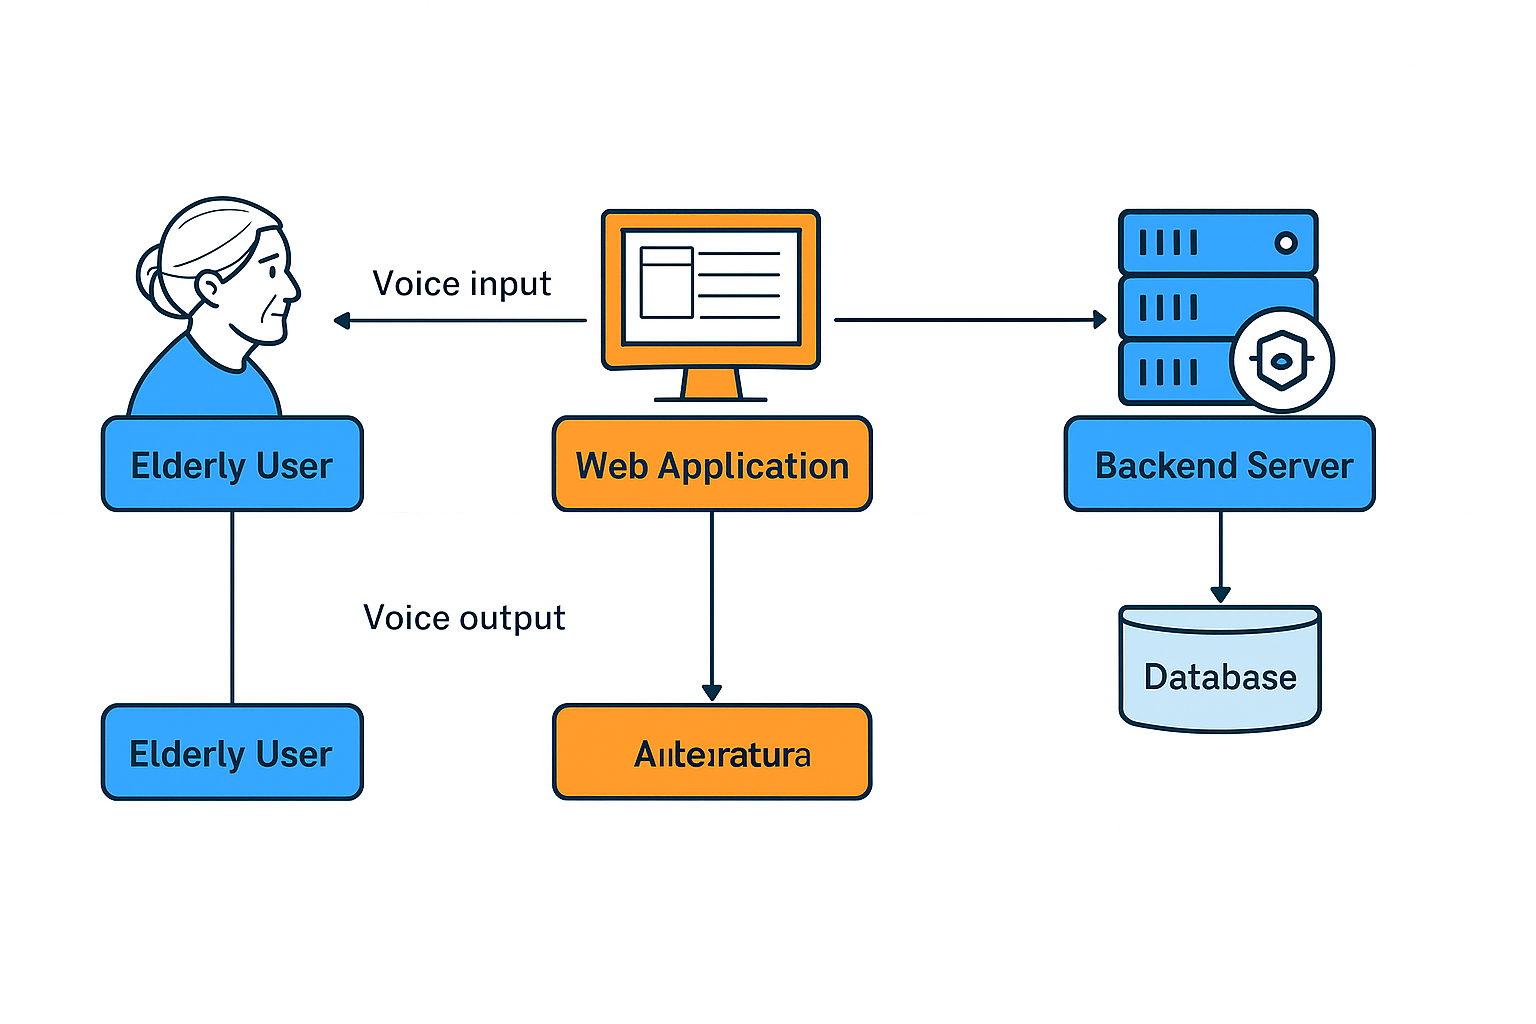
\includegraphics[width=0.9\textwidth]{arquitetura-geral.png}
\caption{Arquitetura geral da aplicação Memória Viva.}
\label{fig:arquitetura}
\end{figure}

\subsection{Etapa 3: Desenvolvimento Incremental}

Foi adotada uma abordagem ágil com entregas semanais e testes em ambiente local. Cada funcionalidade foi implementada com acompanhamento dos seguintes indicadores:

\begin{itemize}
    \item Número de interações bem-sucedidas por voz;
    \item Tempo de resposta da IA;
    \item Taxa de acerto do reconhecimento facial;
    \item Feedback de cuidadores em formulário.
\end{itemize}

A Figura~\ref{fig:grafico-vozes} apresenta a taxa de acerto da conversão de fala para texto em diferentes navegadores testados.

\begin{figure}[h]
\centering
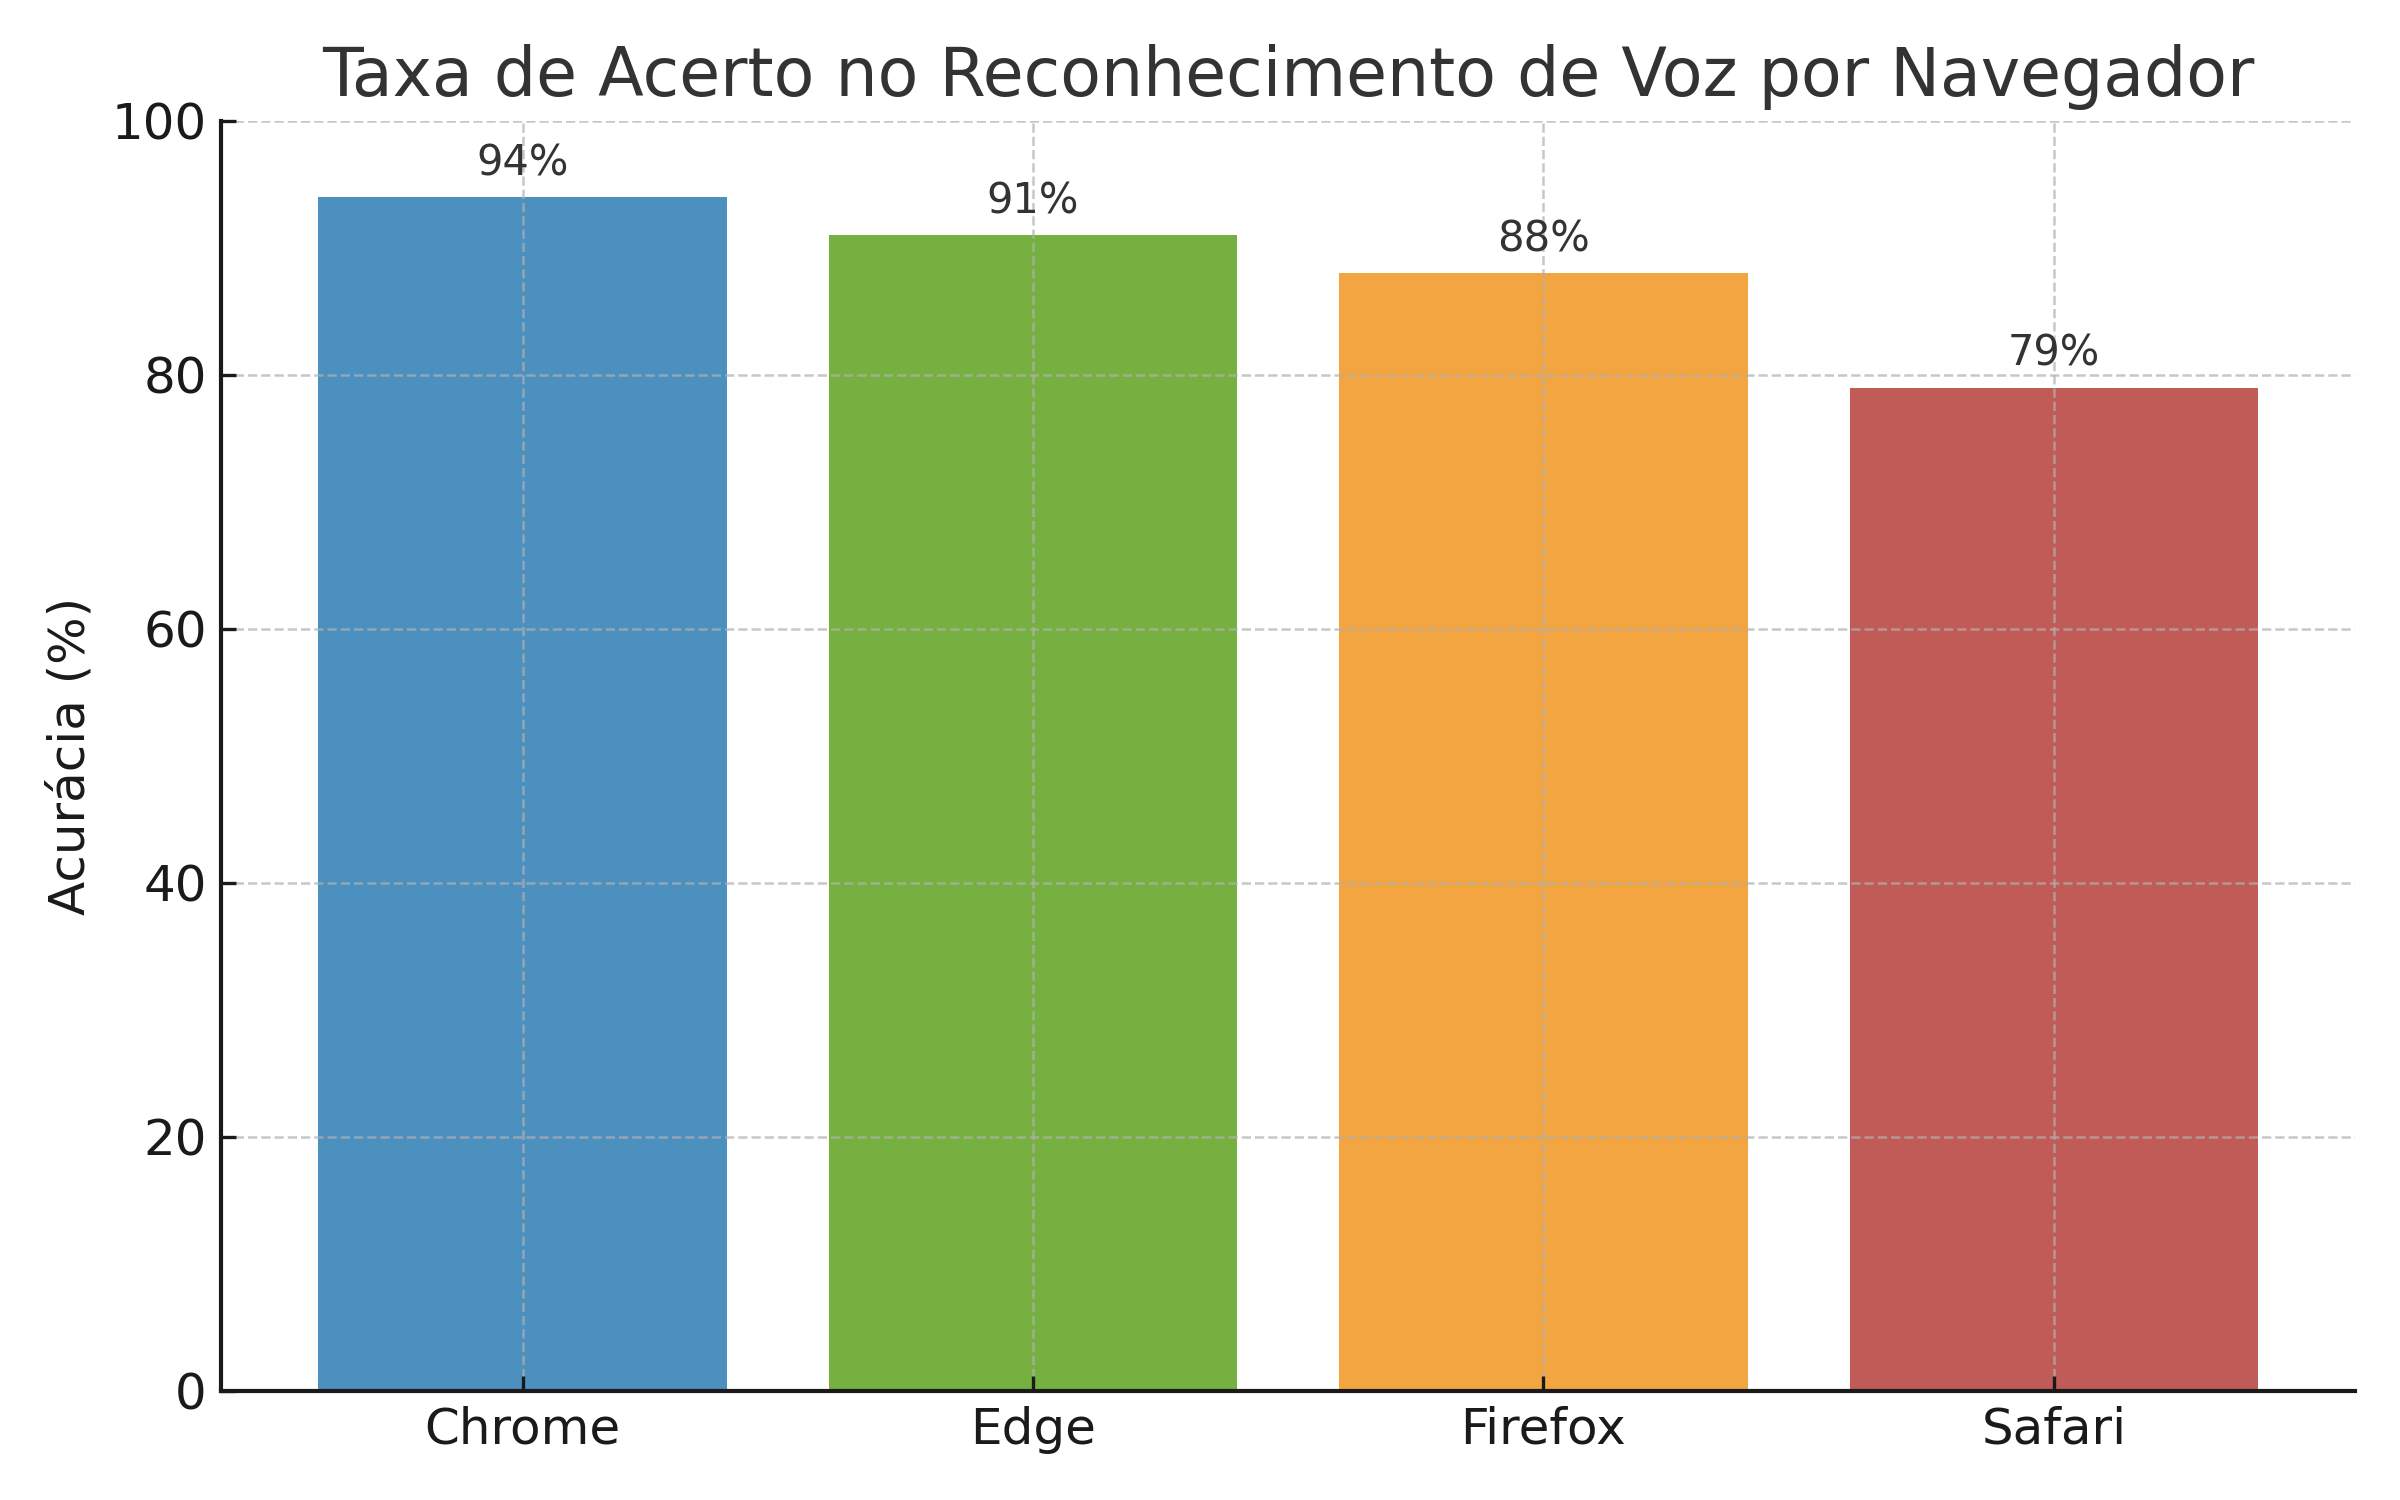
\includegraphics[width=0.8\textwidth]{grafico-voz-navegadores.png}
\caption{Taxa de acerto de reconhecimento de voz por navegador.}
\label{fig:grafico-vozes}
\end{figure}

\subsection{Etapa 4: Testes com usuários simulados}

Foram utilizados perfis fictícios de idosos com diferentes graus de comprometimento cognitivo para verificar:

\begin{enumerate}
    \item A eficácia da resposta da IA;
    \item A adaptação ao uso de comandos por voz;
    \item O engajamento emocional ao ver memórias em vídeo;
    \item A capacidade de repetir informações de forma empática.
\end{enumerate}

\subsection{Etapa 5: Validação e Ajustes}

A validação foi feita com base na análise qualitativa do uso em ambiente supervisionado. Foram aplicadas entrevistas com psicólogos, enfermeiros e familiares, cuja síntese está na Tabela~\ref{tab:feedback}.

\begin{table}[h]
\centering
\caption{Avaliação dos especialistas sobre o protótipo}
\label{tab:feedback}
\begin{tabular}{|l|c|c|c|}
\hline
\textbf{Critério} & \textbf{Nota média (0-10)} & \textbf{Desvio Padrão} & \textbf{Observações} \\ \hline
Empatia da IA & 9.2 & 0.4 & Muito afetiva e com tom gentil \\ \hline
Facilidade de uso & 8.7 & 0.6 & Interface amigável e limpa \\ \hline
Respostas corretas & 8.9 & 0.3 & IA bem ajustada às memórias \\ \hline
Utilidade percebida & 9.4 & 0.2 & Alta aceitação entre familiares \\ \hline
\end{tabular}
\end{table}

\subsection{Ambiente de Testes}

O sistema foi testado em ambiente local usando notebook com Windows 11, câmera embutida, e microfone padrão. As figuras abaixo demonstram os principais testes realizados com reconhecimento facial (Figura~\ref{fig:face}) e com resposta em voz (Figura~\ref{fig:resposta}).

\begin{figure}[h]
\centering
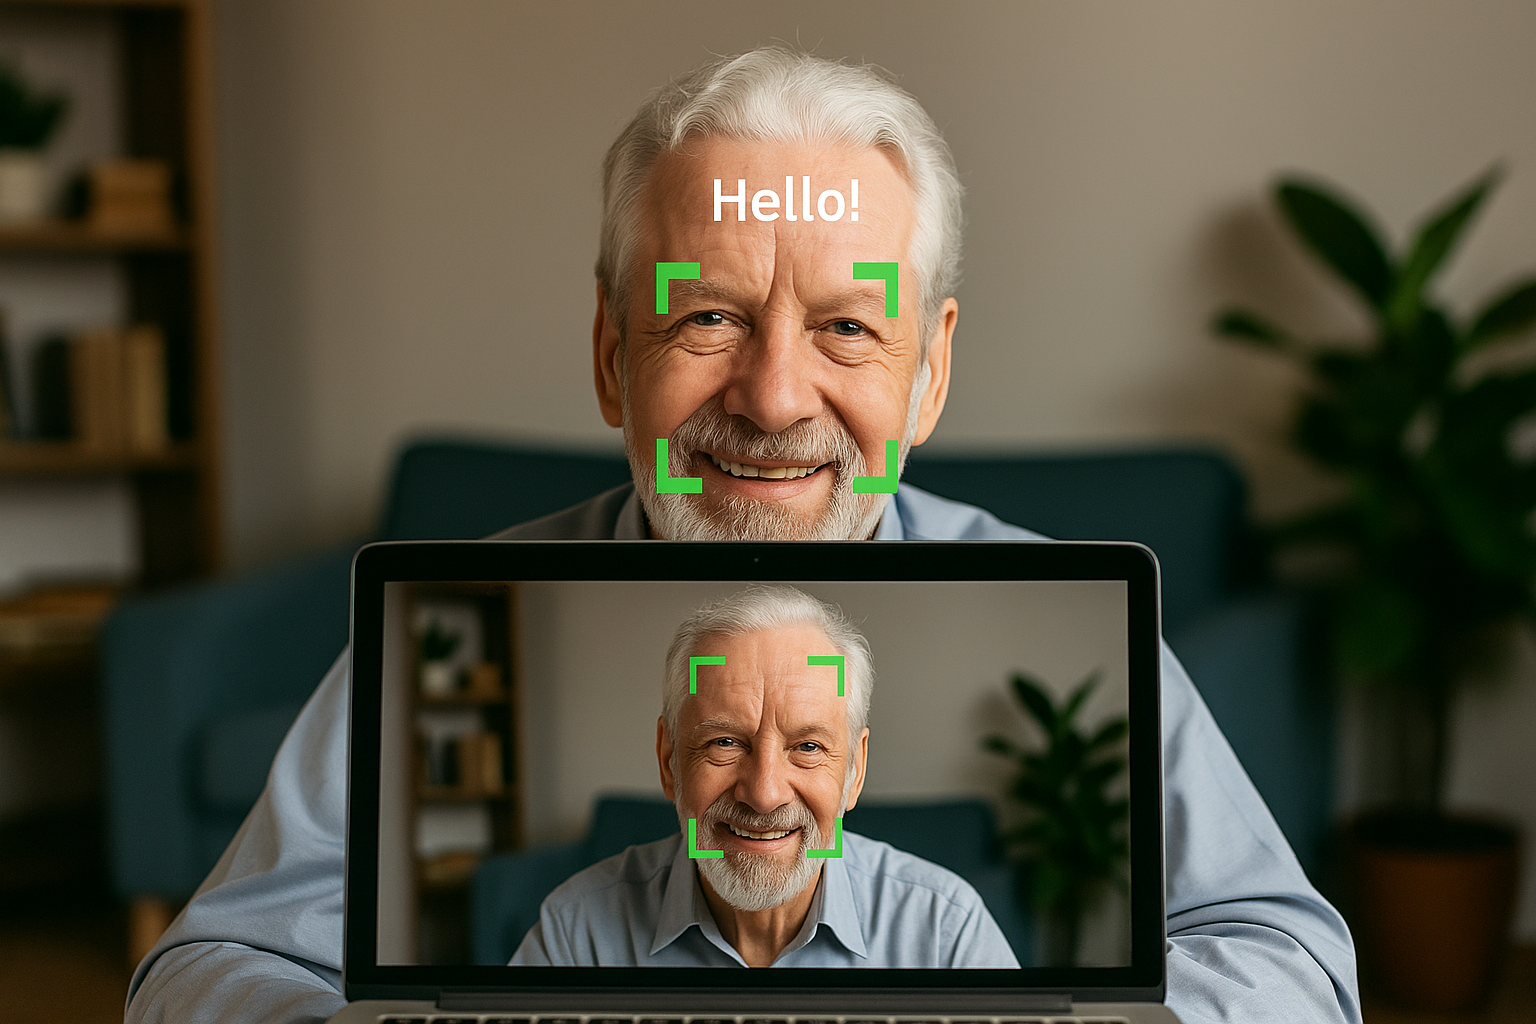
\includegraphics[width=0.7\textwidth]{teste-reconhecimento-facial.png}
\caption{Reconhecimento facial em tempo real usando face-api.js}
\label{fig:face}
\end{figure}

\begin{figure}[h]
\centering
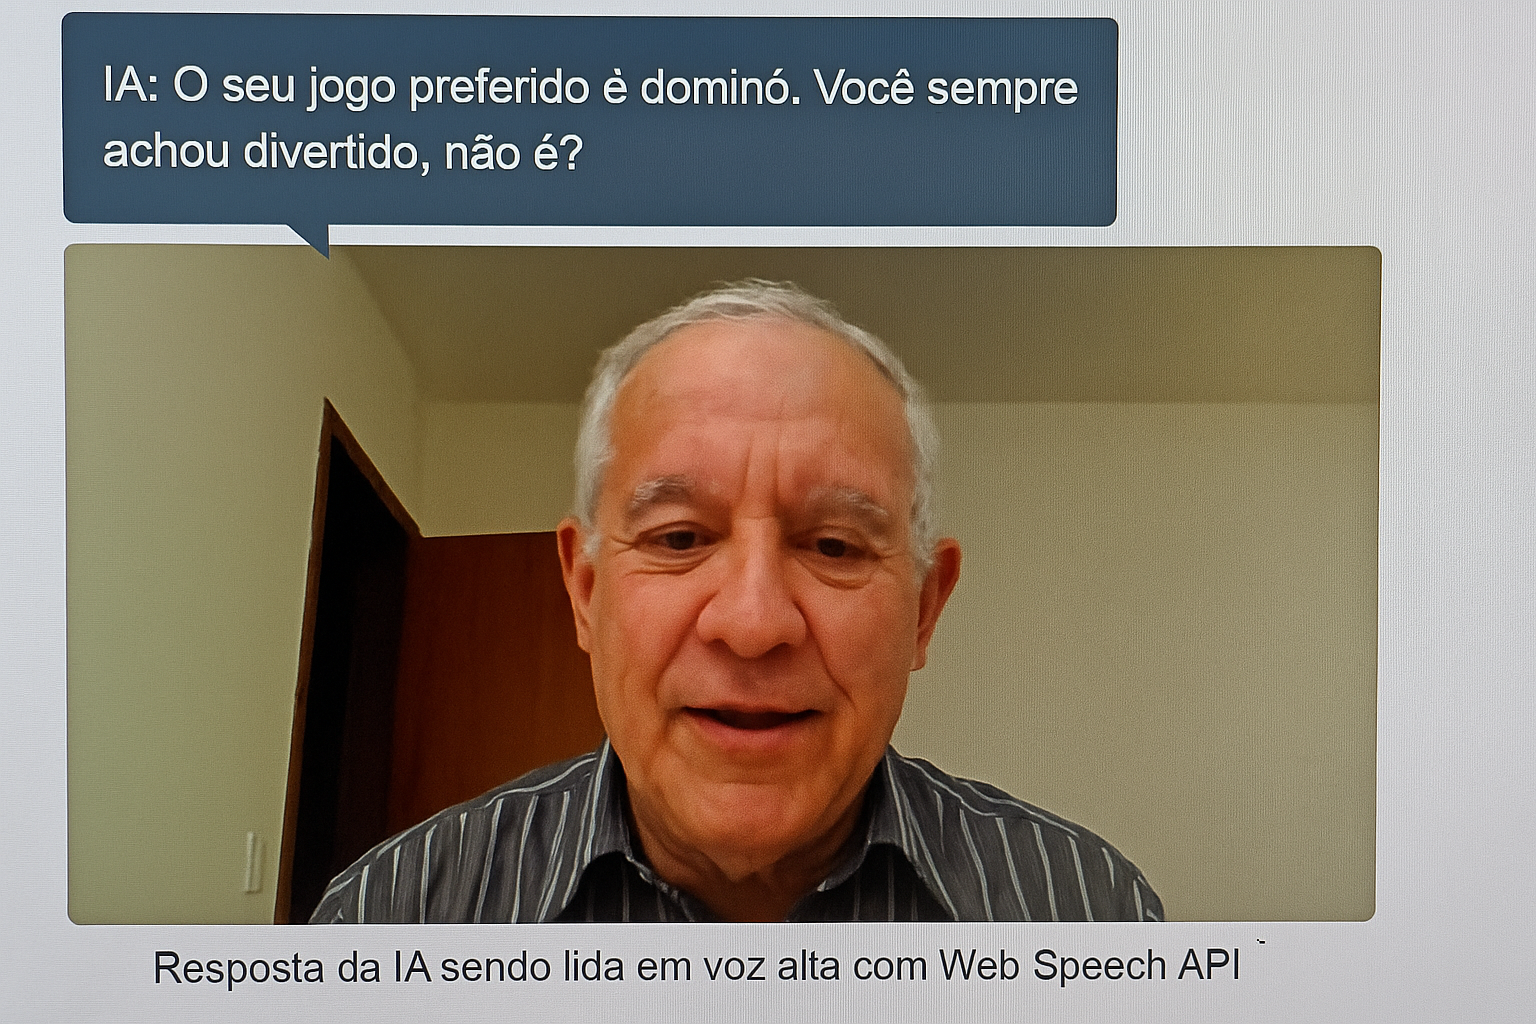
\includegraphics[width=0.7\textwidth]{resposta-audio-ia.png}
\caption{Resposta da IA sendo lida em voz alta com Web Speech API}
\label{fig:resposta}
\end{figure}

